\documentclass[12pt]{article}

\usepackage{graphicx}
\usepackage[margin=1.0in]{geometry}
\usepackage{amsmath}
\usepackage{cases}
\usepackage{amsfonts}
\usepackage{amssymb}
\usepackage{grffile}
\usepackage{setspace}
\usepackage{listings}

\setlength\parindent{0pt}

\author{Xiaohui Chen \\EID: xc2388}
\title{PHY 362K Homework 4}

\begin{document}
\maketitle
\begin{spacing}{2.0}

\section{} %1

\subsection*{(a)}

From this question we know that if there is no perturbation, the Hamiltonian is $H=\frac{\vec{p}^2}{2m^e}- \frac{e^2}{4\pi \epsilon_0 r}$

$\therefore E_n^{(0)}=-\left[ \frac{m}{2\hbar^2} \left( \frac{e^2}{4\pi\epsilon_0} \right)^2 \right] \frac{1}{n^2}$

The perturbed Hamiltonian is $H'=-\mu_{lz}B$

There is no spin, therefore $H'=-\mu_B B\frac{l_z}{\hbar}$ where $\mu_B = \frac{e\hbar}{2m_e}$

Therefore, the first order perturbed Energy, is $E_B^1= \langle H' \rangle = -\frac{\mu_B B}{\hbar} \hbar m_l = -\mu_B B m_l$ where $\mu_B = \frac{e\hbar}{2m_e} \approx 9.273*10^{-24} J/T$

The total energy is $E_{n}= E_n^{(0)}+E_B^1 = -\left[ \frac{m}{2\hbar^2} \left( \frac{e^2}{4\pi\epsilon_0} \right)^2 \right] \frac{1}{n^2} -\mu_B B m_l $

\subsection*{(b)}

\begin{figure}
  \centering
  % Requires \usepackage{graphicx}
  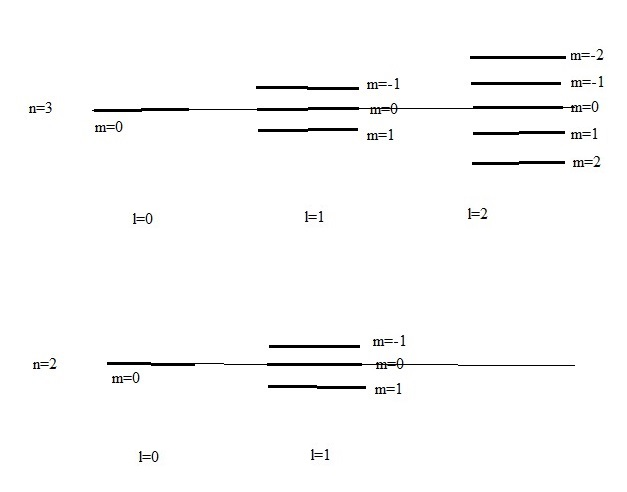
\includegraphics[width=6in]{out1}\\
  \caption{The energy level diagram of "Zeeman energy"}\label{out1}
\end{figure}

The energy level diagram is shown in Figure \ref{out1}. Note that the value between the consecutive spacings is $\mu_B B$

\subsection*{(c)}

\begin{figure}
  \centering
  % Requires \usepackage{graphicx}
  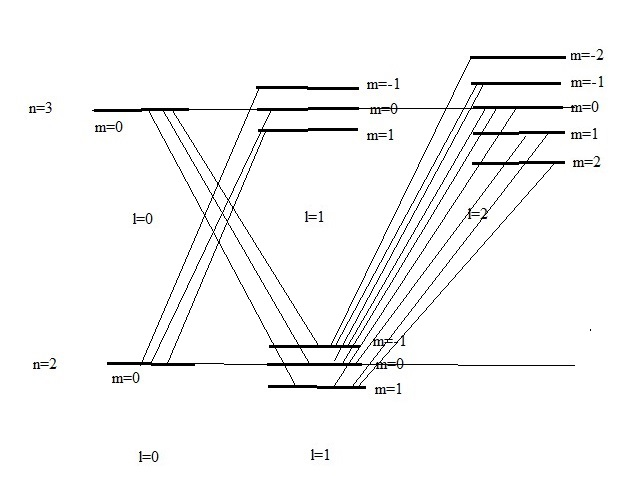
\includegraphics[width=6in]{out2}\\
  \caption{The energy level diagram of "Zeeman energy" with energy transition}\label{out2}
\end{figure}

The allowed transitions are shown in Figure \ref{out2}

\subsection*{(d)}

Since $\Delta l=\pm 1$ and $\Delta m_l=0$ or $\pm 1$, according to the diagram, there are 15 allowed transitions. 

Since There are three distinct energies

$\Delta E_1= -\left[ \frac{m}{2\hbar^2} \left( \frac{e^2}{4\pi\epsilon_0} \right)^2 \right] \left(\frac{1}{3^2}-\frac{1}{2^2}\right) + \mu_B B$ when $\Delta m_l=1$

$\Delta E_2 = -\left[ \frac{m}{2\hbar^2} \left( \frac{e^2}{4\pi\epsilon_0} \right)^2 \right] \left(\frac{1}{3^2}-\frac{1}{2^2}\right) - \mu_B B$ when $\Delta m_l=-1$

$\Delta E_3 = -\left[ \frac{m}{2\hbar^2} \left( \frac{e^2}{4\pi\epsilon_0} \right)^2 \right] \left(\frac{1}{3^2}-\frac{1}{2^2}\right)$ when $\Delta m_l=0$

Therefore there are three distinct frequencies

$f_1=\frac{\Delta E_1}{h}$

$f_2=\frac{\Delta E_2}{h}$

$f_3=\frac{\Delta E_3}{h}$

\begin{figure}
  \centering
  % Requires \usepackage{graphicx}
  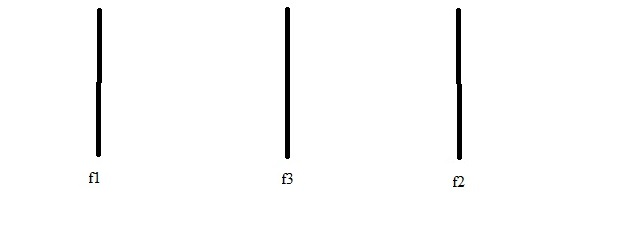
\includegraphics[width=6in]{out3}\\
  \caption{Emission spectrum}\label{out3}
\end{figure}

The spectrum is shown in Figure \ref{out3}

\subsection*{(e)}

When $B=10 T$, the energy spacing is $\Delta E_{Zeeman}= \mu_B B = 9.273*10^{-24}*10 J = 9.273*10^{-23} J$

The wave number is $\bar{v}= \frac{\Delta E_{Zeeman}}{hc}= \frac{9.273*10^{-23}}{6.63*10^{-34}* 3*10^8} *10^{-2} cm^{-1}= 4.66 cm^{-1}$

$\Delta E_{nominal} = -\left[ \frac{m}{2\hbar^2} \left( \frac{e^2}{4\pi\epsilon_0} \right)^2 \right] \left(\frac{1}{3^2}-\frac{1}{2^2}\right)= 13.6*1.6*10^{-19}*\frac{5}{36} J = 3.022*10^{-19} J$

$f_{splitting}=\frac{\Delta E_{Zeeman}}{h}$

$f_{nominal}= \frac{\Delta E_{nominal}}{h}$

$\therefore \frac{f_{splitting}}{f_{nominal}} = \frac{\Delta E_{Zeeman}}{\Delta E_{nominal}} = \frac{9.273*10^{-23}}{3.022*10^{-19}}= 3.068*10^{-4}$

\section{} %2

\subsection*{(a)}

We know that $n=3$ and $s=\frac{1}{2}$. Therefore $j$ can be either $l+\frac{1}{2}$ or $l-\frac{1}{2}$.

We also know that $m_j=-j,-j+1, \ldots, j $

So the possible states are:

$3^2s_{\frac{1}{2},\frac{1}{2}}$, $3^2s_{\frac{1}{2},-\frac{1}{2}}$

$3^2p_{\frac{1}{2},\frac{1}{2}}$, $3^2p_{\frac{1}{2},-\frac{1}{2}}$

$3^2p_{\frac{3}{2},\frac{3}{2}}$, $3^2p_{\frac{3}{2},\frac{1}{2}}$, $3^2p_{\frac{3}{2},-\frac{1}{2}}$, $3^2p_{\frac{3}{2},-\frac{3}{2}}$

$3^2d_{\frac{3}{2},\frac{3}{2}}$, $3^2d_{\frac{3}{2},\frac{1}{2}}$, $3^2d_{\frac{3}{2},-\frac{1}{2}}$, $3^2d_{\frac{3}{2},-\frac{3}{2}}$

$3^2d_{\frac{5}{2},\frac{5}{2}}$, $3^2d_{\frac{5}{2},\frac{3}{2}}$, $3^2d_{\frac{5}{2},\frac{1}{2}}$, $3^2d_{\frac{5}{2},-\frac{1}{2}}$, $3^2d_{\frac{5}{2},-\frac{3}{2}}$, $3^2d_{\frac{5}{2},-\frac{5}{2}}$

\subsection*{(b)}

The states of $|n,l,j,m_j \rangle$ are:

$|3,0,\frac{1}{2},\frac{1}{2} \rangle$, $|3,0,\frac{1}{2},-\frac{1}{2} \rangle$

$|3,1,\frac{1}{2},\frac{1}{2} \rangle$, $|3,1,\frac{1}{2},-\frac{1}{2} \rangle$

$|3,1,\frac{3}{2},\frac{3}{2} \rangle$, $|3,1,\frac{3}{2},\frac{1}{2} \rangle$, $|3,1,\frac{3}{2},-\frac{1}{2} \rangle$, $|3,1,\frac{3}{2},-\frac{3}{2} \rangle$

$|3,2,\frac{3}{2},\frac{3}{2} \rangle$, $|3,2,\frac{3}{2},\frac{1}{2} \rangle$, $|3,2,\frac{3}{2},-\frac{1}{2} \rangle$, $|3,2,\frac{3}{2},-\frac{3}{2} \rangle$

$|3,2,\frac{5}{2},\frac{5}{2} \rangle$, $|3,2,\frac{5}{2},\frac{3}{2} \rangle$, $|3,2,\frac{5}{2},\frac{1}{2} \rangle$, $|3,2,\frac{5}{2},-\frac{1}{2} \rangle$, $|3,2,\frac{5}{2},-\frac{3}{2} \rangle$, $|3,2,\frac{5}{2},-\frac{5}{2} \rangle$



The total number of states is 18, which is the same as the one in part (a)

\subsection*{(c)}

The linear combination is written as $|n,l,m_l,m_s \rangle=\sum_{j=l+s, m_j=m_l+m_s} c_{l,s,m_l,m_s} |l,m_l \rangle |s,m_s\rangle$, where $c_{l,s,m_l,m_s}$ is the coefficient

Using the Clebsch-Gordan coefficients table, we get $|3,2,\frac{3}{2},-\frac{3}{2} \rangle = \sqrt{\frac{1}{5}} |2,-1\rangle |\frac{1}{2},-\frac{1}{2}\rangle -  \sqrt{\frac{4}{5}} |2,-2\rangle |\frac{1}{2},\frac{1}{2}\rangle$

\subsection*{(d)}
Since $m_j=-\frac{3}{2}$, the measurement of $J_z$ is $\hbar m_j=-\frac{3}{2} \hbar$ with possibility 1

\subsection*{(e)}

From part (c) we know that the linear combination is $|3,2,\frac{3}{2},-\frac{3}{2} \rangle = \sqrt{\frac{1}{5}} |2,-1\rangle |\frac{1}{2},-\frac{1}{2}\rangle -  \sqrt{\frac{4}{5}} |2,-2\rangle |\frac{1}{2},\frac{1}{2}\rangle$

The eigenvalue of $L_z$ is $\hbar m_l$

Therefore the measurements are $-\hbar$ with probability $\frac{1}{5}$ and $-2\hbar$ with probability $\frac{4}{5}$

\subsection*{(f)}

The eigenvalue of $S_z$ is $\hbar m_s$

$\therefore \langle S_z \rangle= -\frac{1}{5}* \frac{1}{2} \hbar +\frac{4}{5}*\frac{1}{2} \hbar= \frac{3}{10}\hbar$

\subsection*{(g)}

From the linear combination we can know that $\psi_{r,l,m_l}(r,\theta,\phi)= \sqrt{\frac{1}{5}} R_{32}(r)Y_{2-1}(\theta,\phi) -  \sqrt{\frac{4}{5}} R_{32}(r)Y_{2-2}(\theta,\phi)$

We know that $R_{32}(r)=\frac{4}{81\sqrt{30}}*a_0^{-\frac{3}{2}} \left(\frac{r}{a_0} \right)^2e^{-\frac{r}{3a_0}}$, $Y_{2-1}(\theta,\phi)=\sqrt{\frac{15}{8\pi}}\sin(\theta) \cos(\theta) e^{-i\phi}$ and $Y_{2-2}(\theta,\phi)= \sqrt{\frac{15}{32\pi}}\sin^2(\theta)e^{-2i\phi}$

$a_0=0.5292*10^{-10}$

Plug in the functions above to Mathematica, we get:

$Probability=\psi_{r,l,m_l}(2a_0, \frac{\pi}{3},\frac{\pi}{4})^* \psi_{r,l,m_l}(2a_0, \frac{\pi}{3},\frac{\pi}{4}) (0.002a_0)^3 = 9.5178*10^{-14}$

The Mathematica code is shown below:

\begin{lstlisting}[language=Mathematica,breaklines=true,frame=single]
a0 := 0.5292*10^(-10)
R32[r_] := 4/(81*Sqrt[30]) *a0^(-3/2) *(r/a0)^2*Exp[-r/(3*a0)]
Y2neg1[theta_, phi_] :=
 Sqrt[15/(8*Pi)]*Sin[theta]*Cos[theta]*Exp[-I*phi]
Y2neg2[theta_, phi_] :=
 Sqrt[15/(32*Pi)]*(Sin[theta])^2 * Exp[-2*I*phi]
Psi[r_, theta_, phi_] :=
 Sqrt[1/5]*R32[r]*Y2neg1[theta, phi] -
  Sqrt[4/5]*R32[r]*Y2neg2[theta, phi]
Conjugate[Psi[2*a0, Pi/3, Pi/4]]*Psi[2*a0, Pi/3, Pi/4]*(0.002*a0)^3
\end{lstlisting}

\section{} %3

\subsection*{(a)}
We know that $\vec{j}^2= (\vec{l}+ \vec{s})^2= \vec{l}^2+ 2\vec{l} \cdot\vec{s} + \vec{s}^2$

Therefore $\vec{l} \cdot\vec{s}= \frac{1}{2} (\vec{j}^2 - \vec{l}^2- \vec{s}^2)$

\subsection*{(b)}

The expected value of $\vec{l} \cdot\vec{s}$ is $\langle \vec{l} \cdot\vec{s} \rangle= \frac{1}{2} (\langle \vec{j}^2\rangle - \langle \vec{l}^2\rangle- \langle \vec{s}^2\rangle) = \frac{1}{2}(j(j+1)\hbar^2 - l(l+1)\hbar^2 - s(s+1)\hbar^2) $

Plug in the values of j,l and s in Mathematica, we get

$\vec{l}\cdot \vec{s} =
\left(
\begin{array}{cccccccc}
 0 & 0 & 0 & 0 & 0 & 0 & 0 & 0 \\
 0 & 0 & 0 & 0 & 0 & 0 & 0 & 0 \\
 0 & 0 & -\hbar ^2 & 0 & 0 & 0 & 0 & 0 \\
 0 & 0 & 0 & -\hbar ^2 & 0 & 0 & 0 & 0 \\
 0 & 0 & 0 & 0 & \frac{1}{2}\hbar ^2 & 0 & 0 & 0 \\
 0 & 0 & 0 & 0 & 0 & \frac{1}{2}\hbar ^2 & 0 & 0 \\
 0 & 0 & 0 & 0 & 0 & 0 & \frac{1}{2}\hbar ^2 & 0 \\
 0 & 0 & 0 & 0 & 0 & 0 & 0 & \frac{1}{2}\hbar ^2 \\
\end{array}
\right)$

The Mathematica code is shown below:

\begin{lstlisting}[language=Mathematica,breaklines=true,frame=single]
j := {1/2, 1/2, 1/2, 1/2, 3/2, 3/2, 3/2, 3/2}
l := {0, 0, 1, 1, 1, 1, 1, 1}
s := 1/2
f[x_, y_] :=
 KroneckerDelta[x,
   y]*0.5*((Part[j, x] + 1)*Part[j, x]*\[HBar]^2 - (Part[l, x] + 1)*
     Part[l, x]*\[HBar]^2 - (s + 1)*s*\[HBar]^2)
 
Table[f[x, y], {x, 1, 8}, {y, 1, 8}] // MatrixForm
\end{lstlisting}

\subsection*{(c)}

We know that $l_{\pm}= \vec{l_x} \pm i \vec{l_y} $ and $s_{\pm}= \vec{s_x}\pm i \vec{s_y} $

$\frac{1}{2}(l_+s_- +l_-s_+)+ l_zs_z = \frac{1}{2}[(l_x+il_y)(s_x-is_y) + (l_x-il_y)(s_x+is_y)] + l_zs_z= \frac{1}{2}[l_xs_x -il_xs_y+ il_ys_x + l_ys_y] + l_zs_z= l_xs_x+l_ys_y+l_zs_z= \vec{l}\cdot \vec{s}$

\subsection*{(d)}

The expected value of $\vec{l} \cdot\vec{s}$ is $\frac{1}{2}(j(j+1)\hbar^2 - l(l+1)\hbar^2 - s(s+1)\hbar^2)$

Plug in the values of j,l and s in Mathematica, we get

$\vec{l}\cdot \vec{s} =
\left(
\begin{array}{cccccccc}
 0 & 0 & 0 & 0 & 0 & 0 & 0 & 0 \\
 0 & 0 & 0 & 0 & 0 & 0 & 0 & 0 \\
 0 & 0 & \frac{1}{2}\hbar ^2 & 0 & 0 & 0 & 0 & 0 \\
 0 & 0 & 0 & \frac{1}{2}\hbar ^2 & 0 & 0 & 0 & 0 \\
 0 & 0 & 0 & 0 & \frac{1}{2}\hbar ^2 & 0 & 0 & 0 \\
 0 & 0 & 0 & 0 & 0 & \frac{1}{2}\hbar ^2 & 0 & 0 \\
 0 & 0 & 0 & 0 & 0 & 0 & \frac{1}{2}\hbar ^2 & 0 \\
 0 & 0 & 0 & 0 & 0 & 0 & 0 & \frac{1}{2}\hbar ^2 \\
\end{array}
\right)
$

The Mathematica code is shown below:

\begin{lstlisting}[language=Mathematica,breaklines=true,frame=single]
l1 := {0, 0, 1, 1, 1, 1, 1, 1}
s := 1/2
g[x_, y_] :=
 KroneckerDelta[x,
   y]*0.5*((Part[l1, x] + 1/2 + 1)*(Part[l1, x] +
       1/2)*\[HBar]^2 - (Part[l1, x] + 1)*
     Part[l1, x]*\[HBar]^2 - (s + 1)*s*\[HBar]^2)

Table[g[x, y], {x, 1, 8}, {y, 1, 8}] // MatrixForm
\end{lstlisting}

\section{} %4 6.16

\subsection*{(a)}

$\vec{L}\cdot \vec{S}=L_xS_x+ L_yS_y+ L_zS_z$

$[\vec{L}\cdot \vec{S},L_x]= [L_xS_x+ L_yS_y+ L_zS_z, L_x]= [L_xS_x,Lx]+ [L_yS_y,Lx] + [L_zS_z,Lx] = [L_x,L_x]S_x+ L_x[S_x,L_x]+ L_y[S_y,L_x] +S_y[L_y,L_x] +[L_z,L_x]S_z +L_z[S_z,L_x]= i\hbar L_yS_z - i\hbar L_zS_y = i\hbar(\vec{L}\times \vec{S})_x$

Similarly, we get:

$[\vec{L}\cdot \vec{S},L_y]= [L_xS_x+ L_yS_y+ L_zS_z, L_y]= i\hbar(\vec{L}\times \vec{S})_y$

$[\vec{L}\cdot \vec{S},L_z]= [L_xS_x+ L_yS_y+ L_zS_z, L_z] =i\hbar(\vec{L}\times \vec{S})_z$

According to the three equations above, we get $[\vec{L}\cdot\vec{S}, \vec{L}]= i\hbar(\vec{L}\times \vec{S})$

\subsection*{(b)}

$\vec{L}\cdot \vec{S}=L_xS_x+ L_yS_y+ L_zS_z$

$[\vec{L}\cdot \vec{S},S_x]= [L_xS_x+ L_yS_y+ L_zS_z, S_x]= [L_xS_x,S_x]+ [L_yS_y,S_x] + [L_zS_z,S_x] = [L_x,S_x]S_x+ L_x[S_x,S_x]+ L_y[S_y,S_x] +[L_y,S_x]S_y +[L_z,S_x]S_z +L_z[S_z,S_x]= i\hbar S_yL_z - i\hbar S_zL_y = i\hbar(\vec{S}\times \vec{L})_x$

Similarly, we get:

$[\vec{L}\cdot \vec{S},S_y]= i\hbar(\vec{S}\times \vec{L})_y$

$[\vec{L}\cdot \vec{S},S_z]= i\hbar(\vec{S}\times \vec{L})_z$

According to the three equations above, we get $[\vec{L}\cdot\vec{S}, \vec{S}]= i\hbar(\vec{S}\times \vec{L})$

\subsection*{(c)}

We know that $\vec{J}=\vec{L}+\vec{S}$

Therefore $[\vec{L}\cdot \vec{S},\vec{J}]= [\vec{L}\cdot \vec{S},\vec{L}+ \vec{S}]= [\vec{L}\cdot\vec{S}, \vec{L}] +[\vec{L}\cdot\vec{S}, \vec{S}]= i\hbar(\vec{L}\times \vec{S})+ i\hbar(\vec{S}\times \vec{L}) = i\hbar(\vec{L}\times \vec{S})- i\hbar(\vec{L}\times \vec{S})= 0$

\subsection*{(d)}

Since $L^2$ commutes with all components of $\vec{L}$ and $\vec{S}$, we get: 

$[\vec{L}\cdot \vec{S},L^2]= [L_xS_x+ L_yS_y+ L_zS_z, L^2]= [L_xS_x,Lx]+ [L_yS_y,Lx] + [L_zS_z,Lx] = [L_x,L^2]S_x+ L_x[S_x,L^2]+ L_y[S_y,L^2] +S_y[L_y,L^2] +[L_z,L^2]S_z +L_z[S_z,L^2]= 0$

\subsection*{(e)}

Since $S^2$ commutes with all components of $\vec{L}$ and $\vec{S}$, we get:

$[\vec{L}\cdot \vec{S},S^2]= [L_xS_x+ L_yS_y+ L_zS_z, S^2]= [L_xS_x,Lx]+ [L_yS_y,Lx] + [L_zS_z,Lx] = [L_x,S^2]S_x+ L_x[S_x,S^2]+ L_y[S_y,S^2] +S_y[L_y,S^2] +[L_z,S^2]S_z +L_z[S_z,S^2]= 0$

\subsection*{(f)}

We know that $J^2=L^2+S^2+2\vec{L}\cdot\vec{S}$

$\therefore [\vec{L}\cdot \vec{S},J^2]= [\vec{L}\cdot \vec{S},L^2+S^2+2\vec{L}\cdot\vec{S}]= [\vec{L}\cdot \vec{S},L^2] + [\vec{L}\cdot \vec{S},S^2] +2[\vec{L}\cdot \vec{S},\vec{L}\cdot \vec{S}] = 0$

\section{} %5 6.32

\subsection*{(a)}

$E_n^{(1)}= \langle \psi_n|H'|\psi_n \rangle $

We know that $H=H_0+H'$

We can let $H(\lambda)=H_0$ when $\lambda=\lambda_0$ where $\lambda_0$ is some value

Then $H'=H(\lambda_0+d\lambda)-H_0= H(\lambda_0+d\lambda)- H(\lambda_0)= H d\lambda$ when $\lambda \rightarrow \lambda_0$

Therefore $H'=\frac{\partial H}{\partial \lambda}$

$E_n=E_n^{(0)}+E_n^{(1)}$

By the same approach, we can get $E_n^{1}= E_n d\lambda$ when $\lambda \rightarrow \lambda_0$

Therefore $E_n^{(1)}=\frac{\partial E_n}{\partial \lambda}$

$\therefore \frac{\partial E_n}{\partial \lambda}= \langle \psi_n|\frac{\partial H}{\partial \lambda}|\psi_n \rangle$

\subsection*{(b)}

For an one-dimensional harmonic oscillator, we have:

$H=-\frac{\hbar^2}{2m}\frac{d^2}{dx^2} + \frac{1}{2}m\omega^2x^2$

$T=-\frac{\hbar^2}{2m}\frac{d^2}{dx^2}$

$V=\frac{1}{2}m\omega^2x^2$

$E_n=(n+\frac{1}{2})\hbar \omega$

(i) When $\lambda = \omega$

$\frac{\partial E_n}{\partial \omega}= (n+\frac{1}{2})\hbar$

$\frac{\partial H}{\partial \omega}= m\omega x^2$

Using Feynman-Hellmann theorem:

$\frac{\partial E_n}{\partial \omega}= \langle \psi_n|\frac{\partial H}{\partial \omega}|\psi_n \rangle$

$(n+\frac{1}{2})\hbar = \langle \psi_n|\frac{\partial H}{\partial \omega}|m\omega x^2|\psi_n \rangle$

$\frac{1}{2}(n+\frac{1}{2})\hbar \omega= \langle \psi_n|\frac{\partial H}{\partial \omega}|\frac{1}{2}m\omega^2 x^2|\psi_n \rangle = \langle \psi_n|\frac{\partial H}{\partial \omega}|\frac{1}{2}V|\psi_n \rangle$

$\therefore \langle V \rangle = \frac{1}{2}(n+\frac{1}{2})\hbar \omega$\\

(ii) When $\lambda=\hbar$

$\frac{\partial E_n}{\partial \hbar}= \langle \psi_n|\frac{\partial H}{\partial \hbar}|\psi_n \rangle$

$(n+\frac{1}{2}) \omega= \langle \psi_n|-\frac{\hbar}{m}\frac{d^2}{dx^2}|\psi_n \rangle$

$\frac{\hbar}{2}(n+\frac{1}{2}) \omega= \langle \psi_n|-\frac{\hbar^2}{2m}\frac{d^2}{dx^2}|\psi_n \rangle= \langle \psi_n|T|\psi_n \rangle$

$\therefore \langle T \rangle = \frac{\hbar}{2}(n+\frac{1}{2}) \omega$\\

(iii) When $\lambda=m$

$\frac{\partial E_n}{\partial m}= \langle \psi_n|\frac{\partial H}{\partial m}|\psi_n \rangle$

$0=\langle \psi_n|\frac{\hbar^2}{2m^2}\frac{d^2}{dx^2} + \frac{1}{2} \omega^2 x^2|\psi_n \rangle$

$0=-\frac{1}{m}\langle \psi_n|m\frac{\hbar^2}{2m^2}\frac{d^2}{dx^2} |\psi_n \rangle + \frac{1}{m} \langle \psi_n| m\frac{1}{2} \omega^2 x^2|\psi_n \rangle$

$\langle V \rangle - \langle T \rangle =0 $

$\therefore \langle V \rangle= \langle T \rangle$\\

The results are consistent with Problem 2.12 and Problem 3.31

\section{} %6 6.33

\subsection*{(a)}

We know that $H=-\frac{\hbar^2}{2m} \frac{d^2}{dr^2} + \frac{\hbar^2}{2m} \frac{l(l+1)}{r^2} - \frac{e^2}{4\pi \epsilon_0}\frac{1}{r}$

$E_n=-\frac{me^4}{32\pi^2 \epsilon_0^2 \hbar^2 (j_{max}+l+1)^2}$

Let $\lambda=e$

$\frac{\partial E_n}{\partial e}= \langle \psi_n|\frac{\partial H}{\partial e}|\psi_n \rangle$

$-\frac{me^3}{8\pi^2 \epsilon_0^2 \hbar^2 (j_{max}+l+1)^2}
= \langle \psi_n|
-\frac{e}{2\pi\epsilon_0} \frac{1}{r}
|\psi_n \rangle$

$\frac{me^2}{4\pi \epsilon_0 \hbar^2 (j_{max}+l+1)^2}
= \langle \psi_n|
\frac{1}{r}
|\psi_n \rangle$

$\therefore \langle \frac{1}{r} \rangle = \frac{me^2}{4\pi \epsilon_0 \hbar^2 (j_{max}+l+1)^2} = -\frac{8\pi\epsilon_0}{e^2} E_n = -\frac{8\pi\epsilon_0}{e^2} \frac{E_1}{n^2} = \frac{8\pi\epsilon_0}{e^2n^2} \left[ \frac{m}{2\hbar^2} \left( \frac{e^2}{4\pi\epsilon_0} \right)^2 \right] = \frac{e^2m}{4\pi\epsilon_0\hbar^2}\frac{1}{n^2}$

Let $a_0=\frac{4\pi\epsilon_0 \hbar}{me^2}$, then we get $\langle \frac{1}{r} \rangle = \frac{1}{a_0 n^2}$

\subsection*{(b)}

Let $\lambda=l$

$\frac{\partial E_n}{\partial l}= \langle \psi_n|\frac{\partial H}{\partial l}|\psi_n \rangle$

$\frac{me^4}{16\pi^2 \epsilon_0^2 \hbar^2 = (j_{max}+l+1)^3}
\langle \psi_n|
\frac{\hbar^2}{2m} \frac{2l+1}{r^2}
|\psi_n \rangle$



$\left( -\frac{2}{j_{max}+l+1}E_n \right)=
\left( -\frac{2}{n} \right) E_n=
\langle \psi_n|
\frac{\hbar^2}{2m} \frac{2l+1}{r^2}
|\psi_n \rangle$



$\left( -\frac{2}{j_{max}+l+1} \right) E_n=
\left( -\frac{2}{n} \right) E_n=
\langle \psi_n|
\frac{\hbar^2}{2m} \frac{2l+1}{r^2}
|\psi_n \rangle$

$\therefore \langle \frac{1}{r^2} \rangle= \left( -\frac{4m}{\hbar^2 n(2l+1)} \right) E_n $

Let $a_0=\frac{4\pi\epsilon_0 \hbar}{me^2}$, then we get $\langle \frac{1}{r^2} \rangle = \frac{1}{a_0^2 n^3 \left(l+\frac{1}{2}\right)}$

\end{spacing}
\end{document}